%%
%% This is file `sample-sigconf-authordraft.tex',
%% generated with the docstrip utility.
%%
%% The original source files were:
%%
%% samples.dtx  (with options: `all,proceedings,bibtex,authordraft')
%% 
%% IMPORTANT NOTICE:
%% 
%% For the copyright see the source file.
%% 
%% Any modified versions of this file must be renamed
%% with new filenames distinct from sample-sigconf-authordraft.tex.
%% 
%% For distribution of the original source see the terms
%% for copying and modification in the file samples.dtx.
%% 
%% This generated file may be distributed as long as the
%% original source files, as listed above, are part of the
%% same distribution. (The sources need not necessarily be
%% in the same archive or directory.)
%%
%%
%% Commands for TeXCount
%TC:macro \cite [option:text,text]
%TC:macro \citep [option:text,text]
%TC:macro \citet [option:text,text]
%TC:envir table 0 1
%TC:envir table* 0 1
%TC:envir tabular [ignore] word
%TC:envir displaymath 0 word
%TC:envir math 0 word
%TC:envir comment 0 0
%%
%% The first command in your LaTeX source must be the \documentclass
%% command.
%%
%% For submission and review of your manuscript please change the
%% command to \documentclass[manuscript, screen, review]{acmart}.
%%
%% When submitting camera ready or to TAPS, please change the command
%% to \documentclass[sigconf]{acmart} or whichever template is required
%% for your publication.
%%
%%
\documentclass[sigconf,nonacm]{acmart} % authordraft
%%
%% \BibTeX command to typeset BibTeX logo in the docs
\AtBeginDocument{%
  \providecommand\BibTeX{{%
    Bib\TeX}}}

%% Rights management information.
%% This is a course project report (non-ACM), so we suppress ACM rights and venue metadata.


%%
%% Submission ID.
%% Use this when submitting an article to a sponsored event. You'll
%% receive a unique submission ID from the organizers
%% of the event, and this ID should be used as the parameter to this command.
%%\acmSubmissionID{123-A56-BU3}

%%
%% For managing citations, it is recommended to use bibliography
%% files in BibTeX format.
%%
%% You can then either use BibTeX with the ACM-Reference-Format style,
%% or BibLaTeX with the acmnumeric or acmauthoryear sytles, that include
%% support for advanced citation of software artefact from the
%% biblatex-software package, also separately available on CTAN.
%%
%% Look at the sample-*-biblatex.tex files for templates showcasing
%% the biblatex styles.
%%

%%
%% The majority of ACM publications use numbered citations and
%% references.  The command \citestyle{authoryear} switches to the
%% "author year" style.
%%
%% If you are preparing content for an event
%% sponsored by ACM SIGGRAPH, you must use the "author year" style of
%% citations and references.
%% Uncommenting
%% the next command will enable that style.
%%\citestyle{acmauthoryear}

\settopmatter{printacmref=false}
\renewcommand\footnotetextcopyrightpermission[1]{}
\pagestyle{plain}

%%
%% end of the preamble, start of the body of the document source.
\begin{document}

%%
%% The "title" command has an optional parameter,
%% allowing the author to define a "short title" to be used in page headers.
\title{Do AI Conferences' Ethics Reviews Steer Research Practices?}

%%
%% The "author" command and its associated commands are used to define
%% the authors and their affiliations.
%% Of note is the shared affiliation of the first two authors, and the
%% "authornote" and "authornotemark" commands
%% used to denote shared contribution to the research.
\author{Kento Nishi}
\affiliation{%
  \institution{Harvard University}
  \city{Cambridge}
  \state{MA}
  \country{USA}}
\email{kentonishi@college.harvard.edu}

\author{Alec Laprevotte}
\affiliation{%
  \institution{Harvard University}
  \city{Cambridge}
  \state{MA}
  \country{USA}}
\email{alaprevotte@g.harvard.edu}

\author{Isaiah Bullock}
\affiliation{%
  \institution{Harvard University}
  \city{Cambridge}
  \state{MA}
  \country{USA}}
\email{isaiahabbey@college.harvard.edu}

\author{Mfoniso M. Andrew}
\affiliation{%
  \institution{Harvard University}
  \city{Cambridge}
  \state{MA}
  \country{USA}}
\email{mfonisoandrew@college.harvard.edu}

%%
%% By default, the full list of authors will be used in the page
%% headers. Often, this list is too long, and will overlap
%% other information printed in the page headers. This command allows
%% the author to define a more concise list
%% of authors' names for this purpose.
\renewcommand{\shortauthors}{Nishi et al.}

%%
%% The abstract is a short summary of the work to be presented in the
%% article.
\begin{abstract}
Selective AI/ML conferences increasingly incorporate ethics governance into peer review (ethics flags, impact statements). When reviewers raise ethics concerns and a paper is rejected or withdrawn, authors typically revise and submit elsewhere to a new reviewer pool. Those revisions can be substantive (data, evaluation, scope, release decisions) or rhetorical (expanded limitations and harms framing without changing the technical core). We study these choices by following ICLR 2021--2026 submissions whose reviews included ethics flags into the next public version of the project, and comparing the criticized submission, reviews, and successor paper side by side. Across 47,893 submissions and 185,194 public reviews, we identify 2,498 submissions with reviewer ethics flags, including 1,857 that were rejected or withdrawn. Using OpenAlex-based retrieval, we produced 6,618 candidate successor matches and 601 best-match candidates (not all are true successors). In a first-pass screening of these candidates, we judged 459 pairs likely to describe the same project or a direct descendant; within this screened set, many successors show no observable change or mainly rhetorical change, while a smaller subset show procedural and/or methodological change. We selected 25 stratified cases for author interviews to better understand different views and perspectives on the peer review process. Code will be released upon acceptance.
\end{abstract}

%%
%% The code below is generated by the tool at http://dl.acm.org/ccs.cfm.
%% Please copy and paste the code instead of the example below.
%%
% % \begin{CCSXML}
% % <ccs2012>
% %  <concept>
% %   <concept_id>00000000.0000000.0000000</concept_id>
% %   <concept_desc>Do Not Use This Code, Generate the Correct Terms for Your Paper</concept_desc>
% %   <concept_significance>500</concept_significance>
% %  </concept>
% %  <concept>
% %   <concept_id>00000000.00000000.00000000</concept_id>
% %   <concept_desc>Do Not Use This Code, Generate the Correct Terms for Your Paper</concept_desc>
% %   <concept_significance>300</concept_significance>
% %  </concept>
% %  <concept>
% %   <concept_id>00000000.00000000.00000000</concept_id>
% %   <concept_desc>Do Not Use This Code, Generate the Correct Terms for Your Paper</concept_desc>
% %   <concept_significance>100</concept_significance>
% %  </concept>
% %  <concept>
% %   <concept_id>00000000.00000000.00000000</concept_id>
% %   <concept_desc>Do Not Use This Code, Generate the Correct Terms for Your Paper</concept_desc>
% %   <concept_significance>100</concept_significance>
% %  </concept>
% % </ccs2012>
% % \end{CCSXML}

% \ccsdesc[500]{Do Not Use This Code~Generate the Correct Terms for Your Paper}
% \ccsdesc[300]{Do Not Use This Code~Generate the Correct Terms for Your Paper}
% \ccsdesc{Do Not Use This Code~Generate the Correct Terms for Your Paper}
% \ccsdesc[100]{Do Not Use This Code~Generate the Correct Terms for Your Paper}

%%
%% Keywords. The author(s) should pick words that accurately describe
%% the work being presented. Separate the keywords with commas.
\keywords{AI ethics, peer review, ethics review, research governance, OpenReview}
%% A "teaser" image appears between the author and affiliation
%% information and the body of the document, and typically spans the
%% page.
% \begin{teaserfigure}
%   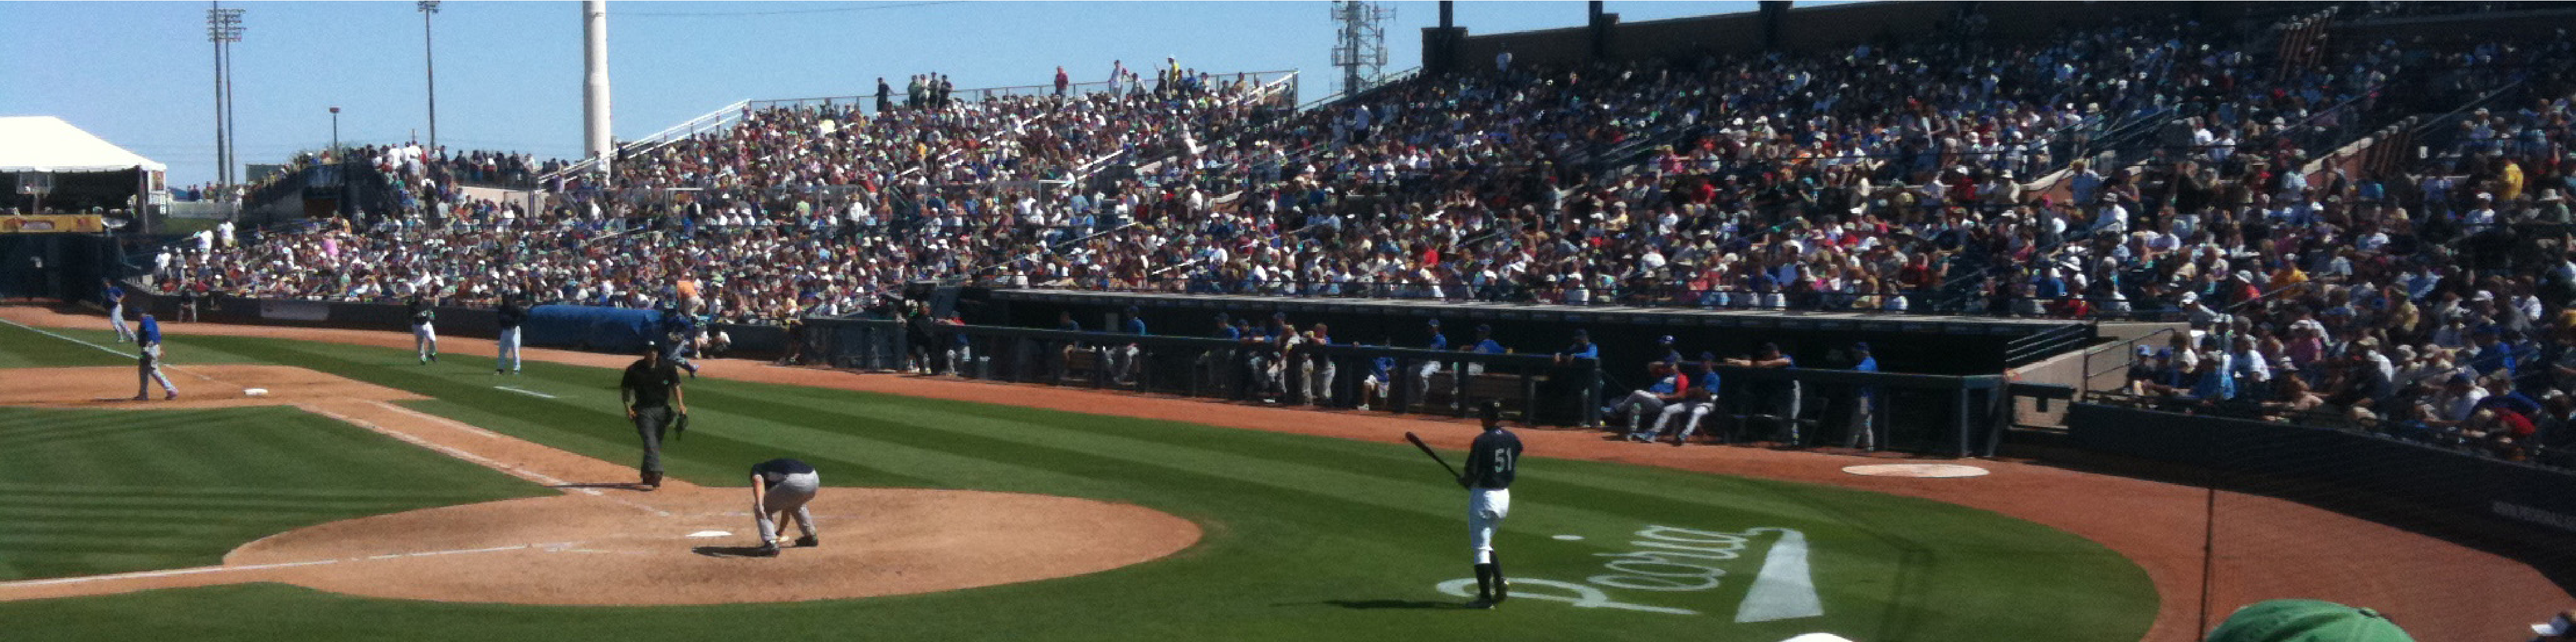
\includegraphics[width=\textwidth]{sampleteaser}
%   \caption{Seattle Mariners at Spring Training, 2010.}
%   \Description{Enjoying the baseball game from the third-base
%   seats. Ichiro Suzuki preparing to bat.}
%   \label{fig:teaser}
% \end{teaserfigure}

% \received{20 February 2007}
% \received[revised]{12 March 2009}
% \received[accepted]{5 June 2009}

%%
%% This command processes the author and affiliation and title
%% information and builds the first part of the formatted document.
\maketitle

\section{Introduction}

In AI and machine learning, selective conferences are primary venues for publishing cutting-edge research. Researchers aim to publish their strongest work at venues such as NeurIPS, ICML, and ICLR, with others often building their next papers on work accepted there. Because acceptance and rejection at these venues affect which projects attract attention and which research directions receive sustained investment, organizers have increasingly extended peer review to include ethical reflection alongside technical evaluation. By the early 2020s, broader impact statements, ethics statements, and reviewer ethics flags had become part of review at these venues \citep{prunkl2021institutionalizing,neurips2021call,neurips2021retrospective,iclr2023ethics}. Reviewers could then raise privacy, fairness, safety, misuse, or deployment concerns alongside technical objections. In many cases, those concerns depended on specific properties of the system under review. For example, \citet{staab2024beyond} show that large language models can infer sensitive personal attributes such as location, income, and sex from real Reddit profiles.

When reviewers criticize a paper on grounds like these, the authors usually do not resubmit their work to the same venue. Instead, they commonly revise their research and submit it to another conference or journal, where a different reviewer pool reads the paper from scratch. Between venues, authors may replace a dataset or add an evaluation, which changes the evidence offered in support of their claims. They may narrow a claim or change whether code or model weights will be released, which changes the scope of the work and the conditions under which other researchers can use it. They may also expand a limitations section, soften claims, or elaborate possible harms, which changes how the work is presented to the next reviewers even when the underlying research process remains the same. These revisions address criticism in different ways: revising data or evaluation changes the research itself, while revising harms and limitations changes how the work is framed for new readers. Because reviewers usually see a paper after much of the technical work is already in place but before the authors settle the version they will submit elsewhere or circulate publicly, the period between one decision and the next submission offers a direct view of what authors chose to change and what they chose to leave alone.

OpenReview publishes the submission, the reviews, the decision, and the associated ethics flags in one public archive. We can therefore read a paper and it's attached criticism concurrently, and once we trace the next public version of the same project, we can compare that earlier criticism with the revisions its authors later made before another submission. Researchers have already used these records to study ethics review inside a single peer review cycle. \citet{liu2022examining} analyze 96 ethics reviews across 50 NeurIPS 2021 papers, the NeurIPS 2021 retrospective reports conditional acceptances and one rejection on ethical grounds, and ICLR 2023 program chairs report screening 190 papers whose reviews included ethics flags before sending a smaller subset for further follow-up \citep{liu2022examining,neurips2021retrospective,iclr2023ethics}. However, these studies focus on a single review cycle and typically do not follow projects into the next submission, when authors decide what a new set of reviewers will see. We therefore follow ICLR submissions whose reviews included ethics flags into later public versions, report preliminary screening results on candidate successor pairs, and conduct interviews with a stratified sample of 25 corresponding authors to clarify why projects changed (or did not) between venues.

\section{Related Work}

\citet{prunkl2021institutionalizing} describe broader impact statements as an attempt to incorporate ethical reflection into ordinary peer review, and they also explain why that arrangement may produce limited change: reviewers may not share standards, authors may face weak incentives, and ethically salient design choices may already be fixed by the time a paper reaches review. Those timing constraints reappear in work on what authors actually wrote under these requirements. For instance, \citet{nanayakkara2021broader} analyze how NeurIPS authors described societal consequences, including how specific those descriptions were and how they handled uncertainty, and \citet{ashurst2022ethics} extend that analysis at larger scale by showing that authors engaged the requirement unevenly. These studies help us read later additions about harms, limitations, and uncertainty as changes in how authors present a paper to readers. However, they do not yet tell us whether the authors changed the underlying research in the same way.

\citet{liu2022examining} are the most directly aligned with our question in their use of public NeurIPS records to analyze how reviewers and authors assigned responsibility for harm and what kinds of revisions reviewers requested. Their analysis remains within a single peer review cycle and does not follow projects into subsequent submissions, where authors decide what to revise, what to defer, what to reframe, and what to leave untouched for a new reviewer pool. That stage is shaped by practical constraints documented in studies of AI work itself. For example, \citet{pant2024ethics} synthesize studies of applied AI practice and report repeated gaps between ethical concern and concrete revision in data practices, evaluation choices, and deployment plans, while \citet{morley2023operationalising} describe similar tensions between general ethical principles and day-to-day engineering constraints. We extend this line of work by comparing criticized submissions with the later papers their authors prepared for another venue, and by interviewing authors about what they changed and why.

\section{Data and Methods}

\subsection{Building the Corpus}

We built the corpus from ICLR because OpenReview publishes the submission, the reviews, the decision, and the associated ethics flags together. From ICLR 2021--2026, we harvested submissions and public replies, normalized titles, abstracts, author lists, decisions, review text, and ethics categories, and then identified papers whose reviews included ethics flags. Because we wanted the corpus to follow the conference's own review process rather than our own retrospective labeling, we used reviewer ethics flags instead of keyword search. We then restricted the corpus to rejected, withdrawn, or unresolved submissions. Accepted ICLR papers had already passed through the venue that issued the criticism. Rejected and withdrawn papers, by contrast, left the authors with a familiar choice in this field: revise the work and send it to another venue. Across the full corpus, we assembled 47,893 submissions and 185,194 public reviews; 2,498 papers had reviews that included ethics flags, and 1,857 of those papers entered the search for later papers. Because the harvested OpenReview snapshot does not expose public ethics flags for ICLR 2021, our ethics-flagged cohort begins in ICLR 2022.

\subsection{Finding Later Versions}

We then searched OpenAlex for later versions of each paper using full titles, title variants, author surnames, and salient abstract terms. Because authors often changed titles, venues, coauthor lists, or project scope after rejection or withdrawal, exact title matching would have missed many plausible later papers. We therefore scored candidates by title similarity, author overlap, abstract overlap, and publication year, kept the highest-scoring candidate for each paper, and saved the larger candidate list whenever the best match remained uncertain. This produced 6,618 candidate successor matches in total and 601 best-match candidates (one per successfully matched rejected/withdrawn paper). We treat these best matches as a starting point for manual validation rather than as ground truth.

\subsection{Reading Pairs and Coding Revision}

Automated retrieval cannot determine whether a later paper truly continues the same project, so successor validation requires reading. We therefore conduct a preliminary screening of candidate pairs to support sampling and planning: for each matched pair, we record whether the later paper appears to be the same project or a direct descendant, and we describe the kinds of changes that are observable between versions (no change, mainly rhetorical change, or procedural/methodological change). We then follow this screening with human-coded validation and inter-rater checks on a subset.

\subsection{Interviewing Authors}

By comparing versions, we can see what changed, but we cannot reliably infer why authors changed one part of a project and left another untouched. We therefore conduct semi-structured interviews with corresponding authors (or designated contacts) from a stratified subset of cases. After receiving staff approval to recruit, we emailed all selected cases on April 14, 2026 and are now scheduling interviews as responses arrive, beginning April 15. Interviews are designed to last approximately 30 minutes. We send the consent form in advance and obtain verbal consent at the start of the call (with a separate prompt for permission to record audio).

Recruitment uses publicly listed contact information associated with the successor paper (e.g., institutional webpages or arXiv metadata). Participation is voluntary, and participants may skip questions or stop at any time. To reduce risk of professional sensitivity, we store recordings and transcripts in access-controlled storage, de-identify transcripts for analysis, and report results in aggregate; if we quote remarks, we anonymize them and review quotations to reduce re-identification risk. Audio recording is optional and, when enabled, is used only to support transcription and analysis.

To complement these interviews with authors, we are also pursuing an interview with a former program chair who has overseen ethics-related review processes, to clarify how ethics flags are used in practice and what constraints chairs face when responding to flagged submissions. We will not ask for or report confidential deliberations about specific submissions.

To keep recruitment consistent and to keep outreach short, we used a standardized email template that introduces the study at a high level, references the public paper pair we traced, and requests a brief call. The template has the following form (with identifying details omitted):
\begin{quote}
\small
Hello \{First name\},

We are conducting a study on how ethics reviews at AI conferences shape papers after ethics-flagged rejections. We saw that your paper ``\{short paper title\}'' was rejected from ICLR \{year\} on the grounds of ethics, but the work is publicly available via \{public venue or archive\}. We would appreciate a brief video call (about 30 minutes) to learn about your rebuttal and resubmission experience, and what (if anything) is different between the ICLR submission and the public version.

If you are willing, please choose a time at \{scheduling link\}. Participation is voluntary; you may decline or stop at any time.

Sincerely, \{research team\}
\end{quote}

\section{Results}

\subsection{Corpus and Candidate Successors}

The number of papers whose reviews included ethics flags rose from 107 in 2022 to 1,100 in 2026, and those flagged papers covered concerns about fairness and discrimination, privacy and safety, harmful applications, legal compliance, responsible research practice, and research integrity. From the 1,857 rejected or withdrawn papers in our corpus, our retrieval produced 601 best-match candidate successors. In a first-pass screening, we judged 459 of the 1,857 rejected/withdrawn cases likely to have a true successor in this best-match set.

For interviews, we selected 25 cases using stratified quotas intended to cover distinct steering relationships and issue areas rather than to estimate population rates. Based on our preliminary screening notes, the sample includes 11 cases in which the successor appears to show especially clear, substantive changes; 6 cases in which ethics-relevant changes were already present in the original submission and the successor largely reflects intrinsic research decisions; and 8 cases in which the flagged concern appears not to be taken up in the successor. We also balanced coverage across four issue areas (harmful applications: 4; fairness/discrimination: 9; responsible research practice: 6; privacy/security/safety: 6). As of April 14, 2026, outreach emails have been sent; interviews are being scheduled as responses arrive, beginning April 15.

\subsection{What Changed in Later Versions}

In our current first-pass screening of the 459 likely successor pairs, 217 successors show no observable change relative to the criticized submission, 153 show mainly rhetorical change (e.g., expanded limitations, harms framing, or responsible-use discussion without technical revision), and a smaller subset show substantive procedural and/or methodological change (57 cases with both procedural and methodological change, 14 with primarily procedural change, and 5 with primarily methodological change). We treat these labels as preliminary: they guide sampling and highlight where deeper reading and inter-rater coding should focus, rather than serving as final measurements.

The substantive changes in our interview sampling set often fall into a few recurring categories. Some successors add dataset curation and quality-control procedures (e.g., explicit leakage checks, majority voting, or volunteer annotation workflows for benchmark construction). Others add additional evaluation and defense analysis (e.g., ablations testing safety finetuning or other mitigations for backdoor and jailbreak-related work). Still others add documentation and governance-relevant detail (e.g., clearer descriptions of consent/IRB in human-subjects settings, dataset cleaning steps to remove identifiers in sensitive domains, or more explicit discussion of data provenance and licensing). By contrast, in unaddressed cases the successor often expands exposition or experiments while leaving the ethics-flagged concern unaddressed in the successor text.

\subsection{Case-specific Interviews}

In the interviews, we ask authors to reconstruct their rebuttal and resubmission experience, what (if anything) is different between the ICLR submission and the later public version, what feedback mattered most, and what constrained revision before the next submission or release. We then ask directly about whether ethics review influenced technical decisions, evaluation choices, release decisions, or only the framing presented to a new reviewer pool. These interviews are designed to clarify when rhetorical revisions reflect strategic reframing versus when they reflect constraints on changing already-implemented systems.

So far, 2 interviews (P1, P2) have been conducted, with 3 more interviews planned. Both interviewees describe first a rejection at ICLR followed by resubmission to a smaller conference where the work was eventually accepted, but they diverge in how much the paper changed and how they interpret the role of peer review.

P1 reports relatively limited substantive change between versions. He describes the later paper as “mostly similar,” with revisions focused on “adding another table,” incorporating “more metrics,” and “fixing the major issues [...] mostly metric based.” He emphasizes frustration with the review process, noting that a reviewer “copied some of the weakness of the previous reviewer without checking if they were actually fixed,” even referencing text that had already been revised. More broadly, he characterizes the process as primarily selective rather than constructive: “the role of peer reviewing [...] is mostly to filter out papers,” and suggests that structural factors such as acceptance rate targets further reinforce this filtering dynamic.

P2, by contrast, describes more extensive revisions following rejection. P2's work was originally meant as an interdisciplinary introduction to highlight his field's overlap with ICLR's focus, but notes that “the paper wasn't written in a way that was clear enough” and that reviewers were “very focused on a particular aspect, [...] instead of seeing a larger picture” . In response, the team “decided to just cut it out completely” (referring the interdisciplinary section), rewrote the introduction for a CS audience, and “recruited 5,000 participants to re-annotate this data set”. Despite accepting many reviewer ethical concerns as “fair points”, he emphasizes that “the criticism is really about my presentation” and that “I don't think [the] review process can actually help the research... it's really about an editorial process” . At the same time, he highlights how this process shapes which contributions are visible: reviewers “have so much power shaping what stories get seen” and in his case, this meant that “it's not as interdisciplinary as you'd like it to be, because the CS reviewers chose to filter it”, effectively using ethics-based rejection to filter the work and influence which kinds of contributions can enter major venues.

\section{Discussion}

Our preliminary screening suggests that ethics-flagged rejected or withdrawn submissions often reappear with limited observable change, and that when changes do appear they are frequently concentrated in framing, limitations, and responsible-use discussion rather than in core methods. Our study design combines manual pair validation with author interviews to characterize which kinds of ethics concerns lead to substantive changes versus rhetorical changes, and what constraints authors report when they choose not to revise the research itself. A plausible hypothesis motivating this design is that reviewer ethics critiques have the most force when they reach parts of a project that authors can still change before the work goes to a different reviewer pool (e.g., scope claims, release plans, or targeted evaluation additions), while changes that require rebuilding a data pipeline or restarting large experimental programs may be less feasible under time and resource constraints.

\subsection{Flawed Reviewers}

Another key aspect from the interviews that was incredibly shocking was the slackness of some reviewers during the reviewing process. The initial idea was focused on rhetoric versus practical change in researchers' work, and through the interviews, there was a shift in direction to questioning the reviewers rather than the researchers. When asked about the reviewing process when submitting to UAI after being declined by ICLR, P1 shared with us that:

\begin{quote}
    \small
    “When I resubmitted this paper, I fixed many things, and the reviewer basically found the ICLR submission, and copied some of the weakness of the previous reviewer without checking if they were actually fixed in the current submission”

\end{quote}
They further confirm this to be true by sharing that the UAI reviewer flagged the submission for the same reason the ICLR reviewer flagged, but the sentence that was flagged was not present in the newer submission where P1 made the necessary adjustments. This reveals that some reviewers are flagging papers to either not have to read them, or to maintain a desired acceptance rate at the conference they are reviewing for.

\section{Limitations}

Our evidence covers only public later papers. Some rejected or withdrawn papers may have changed substantially without leaving a public trace that we could connect to the original submission, and some projects may have split across multiple papers in ways that resist clean reconstruction. Later papers can also absorb feedback from multiple venues, internal lab discussion, legal review, or product constraints, so even a careful pairwise comparison cannot assign every revision to a single source of criticism. We used interviews to address part of that uncertainty, but we still rely on retrospective accounts from people who agreed to speak with us and who reconstructed decisions made under time pressure months or years earlier. We also reduce complicated revision histories to a small set of categories so that we can compare cases systematically. That simplification necessarily drops some detail. For these reasons, we treat our findings as evidence about common patterns in later revision after ethics criticism rather than as definitive causal accounts of every individual paper.

\section{Conclusion}

Selective AI conferences ask reviewers to evaluate ethical concern alongside technical merit, but the consequences of that criticism are only partially visible within a single review cycle. Our approach follows ethics-flagged rejected/withdrawn ICLR submissions into later public versions and uses both document comparisons and author interviews to understand what changed and why. In preliminary screening, many successors show no observable change or mostly rhetorical change, while a smaller subset show procedural and methodological revisions. Ongoing interviews are intended to clarify when those patterns reflect genuine constraints on revision versus strategic choices about what to change and what to present to new reviewers.

% \section{Introduction}
% ACM's consolidated article template, introduced in 2017, provides a
% consistent \LaTeX\ style for use across ACM publications, and
% incorporates accessibility and metadata-extraction functionality
% necessary for future Digital Library endeavors. Numerous ACM and
% SIG-specific \LaTeX\ templates have been examined, and their unique
% features incorporated into this single new template.

% If you are new to publishing with ACM, this document is a valuable
% guide to the process of preparing your work for publication. If you
% have published with ACM before, this document provides insight and
% instruction into more recent changes to the article template.

% The ``\verb|acmart|'' document class can be used to prepare articles
% for any ACM publication --- conference or journal, and for any stage
% of publication, from review to final ``camera-ready'' copy, to the
% author's own version, with {\itshape very} few changes to the source.

% \section{Template Overview}
% As noted in the introduction, the ``\verb|acmart|'' document class can
% be used to prepare many different kinds of documentation --- a
% double-anonymous initial submission of a full-length technical paper, a
% two-page SIGGRAPH Emerging Technologies abstract, a ``camera-ready''
% journal article, a SIGCHI Extended Abstract, and more --- all by
% selecting the appropriate {\itshape template style} and {\itshape
%   template parameters}.

% This document will explain the major features of the document
% class. For further information, the {\itshape \LaTeX\ User's Guide} is
% available from
% \url{https://www.acm.org/publications/proceedings-template}.

% \subsection{Template Styles}

% The primary parameter given to the ``\verb|acmart|'' document class is
% the {\itshape template style} which corresponds to the kind of publication
% or SIG publishing the work. This parameter is enclosed in square
% brackets and is a part of the {\verb|documentclass|} command:
% \begin{verbatim}
%   \documentclass[STYLE]{acmart}
% \end{verbatim}

% Journals use one of three template styles. All but three ACM journals
% use the {\verb|acmsmall|} template style:
% \begin{itemize}
% \item {\texttt{acmsmall}}: The default journal template style.
% \item {\texttt{acmlarge}}: Used by JOCCH and TAP.
% \item {\texttt{acmtog}}: Used by TOG.
% \end{itemize}

% The majority of conference proceedings documentation will use the {\verb|acmconf|} template style.
% \begin{itemize}
% \item {\texttt{sigconf}}: The default proceedings template style.
% \item{\texttt{sigchi}}: Used for SIGCHI conference articles.
% \item{\texttt{sigplan}}: Used for SIGPLAN conference articles.
% \end{itemize}

% \subsection{Template Parameters}

% In addition to specifying the {\itshape template style} to be used in
% formatting your work, there are a number of {\itshape template parameters}
% which modify some part of the applied template style. A complete list
% of these parameters can be found in the {\itshape \LaTeX\ User's Guide.}

% Frequently-used parameters, or combinations of parameters, include:
% \begin{itemize}
% \item {\texttt{anonymous,review}}: Suitable for a ``double-anonymous''
%   conference submission. Anonymizes the work and includes line
%   numbers. Use with the \texttt{\string\acmSubmissionID} command to print the
%   submission's unique ID on each page of the work.
% \item{\texttt{authorversion}}: Produces a version of the work suitable
%   for posting by the author.
% \item{\texttt{screen}}: Produces colored hyperlinks.
% \end{itemize}

% This document uses the following string as the first command in the
% source file:
% \begin{verbatim}
% \documentclass[sigconf,authordraft]{acmart}
% \end{verbatim}

% \section{Modifications}

% Modifying the template --- including but not limited to: adjusting
% margins, typeface sizes, line spacing, paragraph and list definitions,
% and the use of the \verb|\vspace| command to manually adjust the
% vertical spacing between elements of your work --- is not allowed.

% {\bfseries Your document will be returned to you for revision if
%   modifications are discovered.}

% \section{Typefaces}

% The ``\verb|acmart|'' document class requires the use of the
% ``Libertine'' typeface family. Your \TeX\ installation should include
% this set of packages. Please do not substitute other typefaces. The
% ``\verb|lmodern|'' and ``\verb|ltimes|'' packages should not be used,
% as they will override the built-in typeface families.

% \section{Title Information}

% The title of your work should use capital letters appropriately -
% \url{https://capitalizemytitle.com/} has useful rules for
% capitalization. Use the {\verb|title|} command to define the title of
% your work. If your work has a subtitle, define it with the
% {\verb|subtitle|} command.  Do not insert line breaks in your title.

% If your title is lengthy, you must define a short version to be used
% in the page headers, to prevent overlapping text. The \verb|title|
% command has a ``short title'' parameter:
% \begin{verbatim}
%   \title[short title]{full title}
% \end{verbatim}

% \section{Authors and Affiliations}

% Each author must be defined separately for accurate metadata
% identification.  As an exception, multiple authors may share one
% affiliation. Authors' names should not be abbreviated; use full first
% names wherever possible. Include authors' e-mail addresses whenever
% possible.

% Grouping authors' names or e-mail addresses, or providing an ``e-mail
% alias,'' as shown below, is not acceptable:
% \begin{verbatim}
%   \author{Brooke Aster, David Mehldau}
%   \email{dave,judy,steve@university.edu}
%   \email{firstname.lastname@phillips.org}
% \end{verbatim}

% The \verb|authornote| and \verb|authornotemark| commands allow a note
% to apply to multiple authors --- for example, if the first two authors
% of an article contributed equally to the work.

% If your author list is lengthy, you must define a shortened version of
% the list of authors to be used in the page headers, to prevent
% overlapping text. The following command should be placed just after
% the last \verb|\author{}| definition:
% \begin{verbatim}
%   \renewcommand{\shortauthors}{McCartney, et al.}
% \end{verbatim}
% Omitting this command will force the use of a concatenated list of all
% of the authors' names, which may result in overlapping text in the
% page headers.

% The article template's documentation, available at
% \url{https://www.acm.org/publications/proceedings-template}, has a
% complete explanation of these commands and tips for their effective
% use.

% Note that authors' addresses are mandatory for journal articles.

% \section{Rights Information}

% Authors of any work published by ACM will need to complete a rights
% form. Depending on the kind of work, and the rights management choice
% made by the author, this may be copyright transfer, permission,
% license, or an OA (open access) agreement.

% Regardless of the rights management choice, the author will receive a
% copy of the completed rights form once it has been submitted. This
% form contains \LaTeX\ commands that must be copied into the source
% document. When the document source is compiled, these commands and
% their parameters add formatted text to several areas of the final
% document:
% \begin{itemize}
% \item the ``ACM Reference Format'' text on the first page.
% \item the ``rights management'' text on the first page.
% \item the conference information in the page header(s).
% \end{itemize}

% Rights information is unique to the work; if you are preparing several
% works for an event, make sure to use the correct set of commands with
% each of the works.

% The ACM Reference Format text is required for all articles over one
% page in length, and is optional for one-page articles (abstracts).

% \section{CCS Concepts and User-Defined Keywords}

% Two elements of the ``acmart'' document class provide powerful
% taxonomic tools for you to help readers find your work in an online
% search.

% The ACM Computing Classification System ---
% \url{https://www.acm.org/publications/class-2012} --- is a set of
% classifiers and concepts that describe the computing
% discipline. Authors can select entries from this classification
% system, via \url{https://dl.acm.org/ccs/ccs.cfm}, and generate the
% commands to be included in the \LaTeX\ source.

% User-defined keywords are a comma-separated list of words and phrases
% of the authors' choosing, providing a more flexible way of describing
% the research being presented.

% CCS concepts and user-defined keywords are required for for all
% articles over two pages in length, and are optional for one- and
% two-page articles (or abstracts).

% \section{Sectioning Commands}

% Your work should use standard \LaTeX\ sectioning commands:
% \verb|\section|, \verb|\subsection|, \verb|\subsubsection|,
% \verb|\paragraph|, and \verb|\subparagraph|. The sectioning levels up to
% \verb|\subsusection| should be numbered; do not remove the numbering
% from the commands.

% Simulating a sectioning command by setting the first word or words of
% a paragraph in boldface or italicized text is {\bfseries not allowed.}

% Below are examples of sectioning commands.

% \subsection{Subsection}
% \label{sec:subsection}

% This is a subsection.

% \subsubsection{Subsubsection}
% \label{sec:subsubsection}

% This is a subsubsection.

% \paragraph{Paragraph}

% This is a paragraph.

% \subparagraph{Subparagraph}

% This is a subparagraph.

% \section{Tables}

% The ``\verb|acmart|'' document class includes the ``\verb|booktabs|''
% package --- \url{https://ctan.org/pkg/booktabs} --- for preparing
% high-quality tables.

% Table captions are placed {\itshape above} the table.

% Because tables cannot be split across pages, the best placement for
% them is typically the top of the page nearest their initial cite.  To
% ensure this proper ``floating'' placement of tables, use the
% environment \textbf{table} to enclose the table's contents and the
% table caption.  The contents of the table itself must go in the
% \textbf{tabular} environment, to be aligned properly in rows and
% columns, with the desired horizontal and vertical rules.  Again,
% detailed instructions on \textbf{tabular} material are found in the
% \textit{\LaTeX\ User's Guide}.

% Immediately following this sentence is the point at which
% Table~\ref{tab:freq} is included in the input file; compare the
% placement of the table here with the table in the printed output of
% this document.

% \begin{table}
%   \caption{Frequency of Special Characters}
%   \label{tab:freq}
%   \begin{tabular}{ccl}
%     \toprule
%     Non-English or Math&Frequency&Comments\\
%     \midrule
%     \O & 1 in 1,000& For Swedish names\\
%     $\pi$ & 1 in 5& Common in math\\
%     \$ & 4 in 5 & Used in business\\
%     $\Psi^2_1$ & 1 in 40,000& Unexplained usage\\
%   \bottomrule
% \end{tabular}
% \end{table}

% To set a wider table, which takes up the whole width of the page's
% live area, use the environment \textbf{table*} to enclose the table's
% contents and the table caption.  As with a single-column table, this
% wide table will ``float'' to a location deemed more
% desirable. Immediately following this sentence is the point at which
% Table~\ref{tab:commands} is included in the input file; again, it is
% instructive to compare the placement of the table here with the table
% in the printed output of this document.

% \begin{table*}
%   \caption{Some Typical Commands}
%   \label{tab:commands}
%   \begin{tabular}{ccl}
%     \toprule
%     Command &A Number & Comments\\
%     \midrule
%     \texttt{{\char'134}author} & 100& Author \\
%     \texttt{{\char'134}table}& 300 & For tables\\
%     \texttt{{\char'134}table*}& 400& For wider tables\\
%     \bottomrule
%   \end{tabular}
% \end{table*}

% Always use midrule to separate table header rows from data rows, and
% use it only for this purpose. This enables assistive technologies to
% recognise table headers and support their users in navigating tables
% more easily.

% \section{Math Equations}
% You may want to display math equations in three distinct styles:
% inline, numbered or non-numbered display.  Each of the three are
% discussed in the next sections.

% \subsection{Inline (In-text) Equations}
% A formula that appears in the running text is called an inline or
% in-text formula.  It is produced by the \textbf{math} environment,
% which can be invoked with the usual
% \texttt{{\char'134}begin\,\ldots{\char'134}end} construction or with
% the short form \texttt{\$\,\ldots\$}. You can use any of the symbols
% and structures, from $\alpha$ to $\omega$, available in
% \LaTeX~\cite{Lamport:LaTeX}; this section will simply show a few
% examples of in-text equations in context. Notice how this equation:
% \begin{math}
%   \lim_{n\rightarrow \infty}x=0
% \end{math},
% set here in in-line math style, looks slightly different when
% set in display style.  (See next section).

% \subsection{Display Equations}
% A numbered display equation---one set off by vertical space from the
% text and centered horizontally---is produced by the \textbf{equation}
% environment. An unnumbered display equation is produced by the
% \textbf{displaymath} environment.

% Again, in either environment, you can use any of the symbols and
% structures available in \LaTeX\@; this section will just give a couple
% of examples of display equations in context.  First, consider the
% equation, shown as an inline equation above:
% \begin{equation}
%   \lim_{n\rightarrow \infty}x=0
% \end{equation}
% Notice how it is formatted somewhat differently in
% the \textbf{displaymath}
% environment.  Now, we'll enter an unnumbered equation:
% \begin{displaymath}
%   \sum_{i=0}^{\infty} x + 1
% \end{displaymath}
% and follow it with another numbered equation:
% \begin{equation}
%   \sum_{i=0}^{\infty}x_i=\int_{0}^{\pi+2} f
% \end{equation}
% just to demonstrate \LaTeX's able handling of numbering.

% \section{Figures}

% The ``\verb|figure|'' environment should be used for figures. One or
% more images can be placed within a figure. If your figure contains
% third-party material, you must clearly identify it as such, as shown
% in the example below.
% \begin{figure}[h]
%   \centering
%   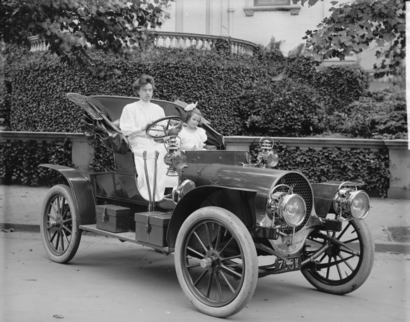
\includegraphics[width=\linewidth]{sample-franklin}
%   \caption{1907 Franklin Model D roadster. Photograph by Harris \&
%     Ewing, Inc. [Public domain], via Wikimedia
%     Commons. (\url{https://goo.gl/VLCRBB}).}
%   \Description{A woman and a girl in white dresses sit in an open car.}
% \end{figure}

% Your figures should contain a caption which describes the figure to
% the reader.

% Figure captions are placed {\itshape below} the figure.

% Every figure should also have a figure description unless it is purely
% decorative. These descriptions convey what’s in the image to someone
% who cannot see it. They are also used by search engine crawlers for
% indexing images, and when images cannot be loaded.

% A figure description must be unformatted plain text less than 2000
% characters long (including spaces).  {\bfseries Figure descriptions
%   should not repeat the figure caption – their purpose is to capture
%   important information that is not already provided in the caption or
%   the main text of the paper.} For figures that convey important and
% complex new information, a short text description may not be
% adequate. More complex alternative descriptions can be placed in an
% appendix and referenced in a short figure description. For example,
% provide a data table capturing the information in a bar chart, or a
% structured list representing a graph.  For additional information
% regarding how best to write figure descriptions and why doing this is
% so important, please see
% \url{https://www.acm.org/publications/taps/describing-figures/}.

% \subsection{The ``Teaser Figure''}

% A ``teaser figure'' is an image, or set of images in one figure, that
% are placed after all author and affiliation information, and before
% the body of the article, spanning the page. If you wish to have such a
% figure in your article, place the command immediately before the
% \verb|\maketitle| command:
% \begin{verbatim}
%   \begin{teaserfigure}
%     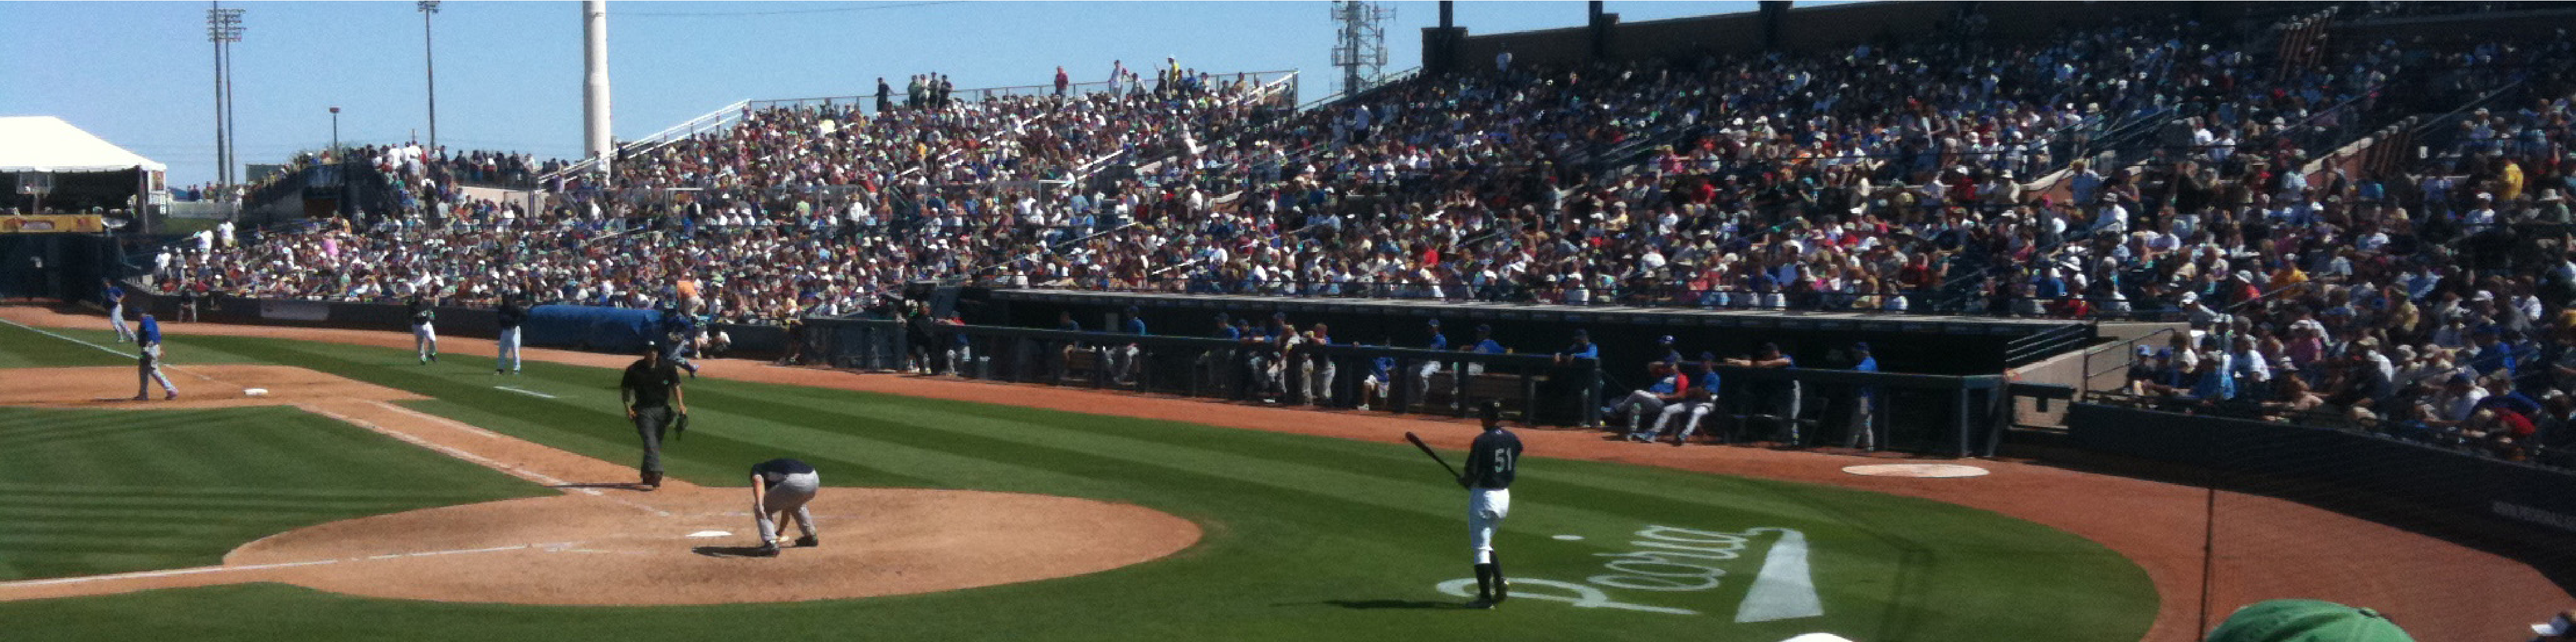
\includegraphics[width=\textwidth]{sampleteaser}
%     \caption{figure caption}
%     \Description{figure description}
%   \end{teaserfigure}
% \end{verbatim}

% \section{Citations and Bibliographies}

% The use of \BibTeX\ for the preparation and formatting of one's
% references is strongly recommended. Authors' names should be complete
% --- use full first names (``Donald E. Knuth'') not initials
% (``D. E. Knuth'') --- and the salient identifying features of a
% reference should be included: title, year, volume, number, pages,
% article DOI, etc.

% The bibliography is included in your source document with these two
% commands, placed just before the \verb|\end{document}| command:
% \begin{verbatim}
%   \bibliographystyle{ACM-Reference-Format}
%   \bibliography{bibfile}
% \end{verbatim}
% where ``\verb|bibfile|'' is the name, without the ``\verb|.bib|''
% suffix, of the \BibTeX\ file.

% Citations and references are numbered by default. A small number of
% ACM publications have citations and references formatted in the
% ``author year'' style; for these exceptions, please include this
% command in the {\bfseries preamble} (before the command
% ``\verb|\begin{document}|'') of your \LaTeX\ source:
% \begin{verbatim}
%   \citestyle{acmauthoryear}
% \end{verbatim}


%   Some examples.  A paginated journal article \cite{Abril07}, an
%   enumerated journal article \cite{Cohen07}, a reference to an entire
%   issue \cite{JCohen96}, a monograph (whole book) \cite{Kosiur01}, a
%   monograph/whole book in a series (see 2a in spec. document)
%   \cite{Harel79}, a divisible-book such as an anthology or compilation
%   \cite{Editor00} followed by the same example, however we only output
%   the series if the volume number is given \cite{Editor00a} (so
%   Editor00a's series should NOT be present since it has no vol. no.),
%   a chapter in a divisible book \cite{Spector90}, a chapter in a
%   divisible book in a series \cite{Douglass98}, a multi-volume work as
%   book \cite{Knuth97}, a couple of articles in a proceedings (of a
%   conference, symposium, workshop for example) (paginated proceedings
%   article) \cite{Andler79, Hagerup1993}, a proceedings article with
%   all possible elements \cite{Smith10}, an example of an enumerated
%   proceedings article \cite{VanGundy07}, an informally published work
%   \cite{Harel78}, a couple of preprints \cite{Bornmann2019,
%     AnzarootPBM14}, a doctoral dissertation \cite{Clarkson85}, a
%   master's thesis: \cite{anisi03}, an online document / world wide web
%   resource \cite{Thornburg01, Ablamowicz07, Poker06}, a video game
%   (Case 1) \cite{Obama08} and (Case 2) \cite{Novak03} and \cite{Lee05}
%   and (Case 3) a patent \cite{JoeScientist001}, work accepted for
%   publication \cite{rous08}, 'YYYYb'-test for prolific author
%   \cite{SaeediMEJ10} and \cite{SaeediJETC10}. Other cites might
%   contain 'duplicate' DOI and URLs (some SIAM articles)
%   \cite{Kirschmer:2010:AEI:1958016.1958018}. Boris / Barbara Beeton:
%   multi-volume works as books \cite{MR781536} and \cite{MR781537}. A
%   presentation~\cite{Reiser2014}. An article under
%   review~\cite{Baggett2025}. A
%   couple of citations with DOIs:
%   \cite{2004:ITE:1009386.1010128,Kirschmer:2010:AEI:1958016.1958018}. Online
%   citations: \cite{TUGInstmem, Thornburg01, CTANacmart}.
%   Artifacts: \cite{R} and \cite{UMassCitations}.

% \section{Acknowledgments}

% Identification of funding sources and other support, and thanks to
% individuals and groups that assisted in the research and the
% preparation of the work should be included in an acknowledgment
% section, which is placed just before the reference section in your
% document.

% This section has a special environment:
% \begin{verbatim}
%   \begin{acks}
%   ...
%   \end{acks}
% \end{verbatim}
% so that the information contained therein can be more easily collected
% during the article metadata extraction phase, and to ensure
% consistency in the spelling of the section heading.

% Authors should not prepare this section as a numbered or unnumbered {\verb|\section|}; please use the ``{\verb|acks|}'' environment.

% \section{Appendices}

% If your work needs an appendix, add it before the
% ``\verb|\end{document}|'' command at the conclusion of your source
% document.

% Start the appendix with the ``\verb|appendix|'' command:
% \begin{verbatim}
%   \appendix
% \end{verbatim}
% and note that in the appendix, sections are lettered, not
% numbered. This document has two appendices, demonstrating the section
% and subsection identification method.

% \section{Multi-language papers}

% Papers may be written in languages other than English or include
% titles, subtitles, keywords and abstracts in different languages (as a
% rule, a paper in a language other than English should include an
% English title and an English abstract).  Use \verb|language=...| for
% every language used in the paper.  The last language indicated is the
% main language of the paper.  For example, a French paper with
% additional titles and abstracts in English and German may start with
% the following command
% \begin{verbatim}
% \documentclass[sigconf, language=english, language=german,
%                language=french]{acmart}
% \end{verbatim}

% The title, subtitle, keywords and abstract will be typeset in the main
% language of the paper.  The commands \verb|\translatedXXX|, \verb|XXX|
% begin title, subtitle and keywords, can be used to set these elements
% in the other languages.  The environment \verb|translatedabstract| is
% used to set the translation of the abstract.  These commands and
% environment have a mandatory first argument: the language of the
% second argument.  See \verb|sample-sigconf-i13n.tex| file for examples
% of their usage.

% \section{SIGCHI Extended Abstracts}

% The ``\verb|sigchi-a|'' template style (available only in \LaTeX\ and
% not in Word) produces a landscape-orientation formatted article, with
% a wide left margin. Three environments are available for use with the
% ``\verb|sigchi-a|'' template style, and produce formatted output in
% the margin:
% \begin{description}
% \item[\texttt{sidebar}:]  Place formatted text in the margin.
% \item[\texttt{marginfigure}:] Place a figure in the margin.
% \item[\texttt{margintable}:] Place a table in the margin.
% \end{description}

% %%
% %% The acknowledgments section is defined using the "acks" environment
% %% (and NOT an unnumbered section). This ensures the proper
% %% identification of the section in the article metadata, and the
% %% consistent spelling of the heading.
% \begin{acks}
% To Robert, for the bagels and explaining CMYK and color spaces.
% \end{acks}

% %%
% %% The next two lines define the bibliography style to be used, and
% %% the bibliography file.
% \bibliographystyle{ACM-Reference-Format}
% \bibliography{sample-base}


% %%
% %% If your work has an appendix, this is the place to put it.
% \appendix

% \section{Research Methods}

% \subsection{Part One}

% Lorem ipsum dolor sit amet, consectetur adipiscing elit. Morbi
% malesuada, quam in pulvinar varius, metus nunc fermentum urna, id
% sollicitudin purus odio sit amet enim. Aliquam ullamcorper eu ipsum
% vel mollis. Curabitur quis dictum nisl. Phasellus vel semper risus, et
% lacinia dolor. Integer ultricies commodo sem nec semper.

% \subsection{Part Two}

% Etiam commodo feugiat nisl pulvinar pellentesque. Etiam auctor sodales
% ligula, non varius nibh pulvinar semper. Suspendisse nec lectus non
% ipsum convallis congue hendrerit vitae sapien. Donec at laoreet
% eros. Vivamus non purus placerat, scelerisque diam eu, cursus
% ante. Etiam aliquam tortor auctor efficitur mattis.

% \section{Online Resources}

% Nam id fermentum dui. Suspendisse sagittis tortor a nulla mollis, in
% pulvinar ex pretium. Sed interdum orci quis metus euismod, et sagittis
% enim maximus. Vestibulum gravida massa ut felis suscipit
% congue. Quisque mattis elit a risus ultrices commodo venenatis eget
% dui. Etiam sagittis eleifend elementum.

% Nam interdum magna at lectus dignissim, ac dignissim lorem
% rhoncus. Maecenas eu arcu ac neque placerat aliquam. Nunc pulvinar
% massa et mattis lacinia.

\bibliographystyle{ACM-Reference-Format}
\bibliography{references}
\end{document}
\endinput
%%
%% End of file `sample-sigconf-authordraft.tex'.
